\documentclass[sigplan,screen]{acmart}

%\hyphenation{globally-asyn-chronous}

%\usepackage{listings}
\usepackage{xspace}
\newcommand{\lin}[1]{(\emph{ln. #1}\xspace)}
\newcommand{\dapp}{\emph{dapp}\xspace}
\newcommand{\dapps}{\emph{dapps}\xspace}

\setcopyright{acmcopyright}
\copyrightyear{2018}
\acmYear{2018}
\acmDOI{10.1145/1122445.1122456}

\acmConference[REBLS '21]{REBLS '21: ACM Workshop on Reactive and Event-Based Languages and Systems}{June 03--05, 2018}{Chicago, IL}
\acmBooktitle{REBLS '21: ACM Workshop on Reactive and Event-Based Languages and Systems, June 03--05, 2018, Chicago, IL}
\acmPrice{15.00}
\acmISBN{978-1-4503-XXXX-X/18/06}

%\acmSubmissionID{123-A56-BU3}
%\citestyle{acmauthoryear}

\begin{document}

\title{Symmetric Distributed Applications}

\author{Francisco Sant'Anna}
\email{francisco@ime.uerj.br}
%\orcid{1234-5678-9012}
\affiliation{%
  \institution{Rio de Janeiro State University (UERJ)}
  \country{Brazil}
}

\author{Rodrigo Santos}
\email{rodsantos@microsoft.com}
\affiliation{%
  \institution{Microsoft}
  \country{Brazil}
}

\author{Noemi Rodriguez}
\email{noemi@inf.puc-rio.br}
\affiliation{%
  \institution{PUC-Rio}
  \country{Brazil}
}

%\renewcommand{\shortauthors}{Trovato and Tobin, et al.}

\begin{abstract}
A program is deterministic if multiple re-executions with the same inputs
always lead to the same state.
Even concurrent instances of a deterministic program should observe identical
behavior---in real time---if assigned the same set of inputs.
%
In this work, we propose real-time reproducibility for distributed programs.
Multiple instances of the same interactive application can broadcast
asynchronous inputs and yet conform to identical behavior.
Collaborative networked applications, such as watch parties, document editing,
and video games can benefit from this approach.
We name this class of applications as \emph{symmetric distributed applications}.
%
Using a standard event-driven API to wait and emit events, programmers write
code as if the application executes in a single machine.
Our middleware intercepts event generation and synchronizes all instances in a
consistent timeline so that receipt is identically reproducible.
Not only distributed applications benefit from consistency and determinism but
also development and testing can be done in a single instance with the same
guarantees.
In our experiments, the middleware can handle applications with 25 FPS,
distributed in up to 25 nodes over the Internet, with an event latency below
$350ms$.
\end{abstract}

\begin{comment}
\begin{CCSXML}
<ccs2012>
 <concept>
  <concept_id>10003033.10003083.10003095</concept_id>
  <concept_desc>Networks~Network reliability</concept_desc>
  <concept_significance>100</concept_significance>
 </concept>
</ccs2012>
\end{CCSXML}
\ccsdesc[100]{Networks~Network reliability}
\end{comment}

\keywords{consistency, determinism, GALS, synchronous programming, distributed applications}

\maketitle

\section{Introduction}

Deterministic programs are easier to understand, test, and verify~\cite{det}.
Considering unpredictable user interactions, a program is deterministic if
re-execution with the same order and timing of inputs always leads to the same
state.
With such timeline reproducibility property, multiple re-executions are
indistinguishable from each other.
Considering now distribution, it should be possible to provide a
sequentially consistent timeline to concurrent instances of a deterministic
program and also observe identical behavior \emph{in real time}.

In this work, our goal is to support the real-time reproducibility property in
a distributed setting.
We propose that mirrored instances of the same application running in different
machines should be able to broadcast asynchronous inputs to each other and yet
conform to identical behavior.
Hence, our focus is on \emph{symmetric distributed applications}, instead of
machines playing different roles in the network.
A programmer writes the intended distributed application as if it would execute
in a single machine.
The underlying system we propose supports distribution and guarantees a
sequentially consistent timeline to all instances, which react to this timeline
deterministically.
Hence, we support determinism locally at individual instances, and consistency
globally at the whole distributed system level.

Collaborative networked applications fall in the class of symmetric
distribution and can benefit from transparent reproducibility.
As an example, \emph{watch parties} are social gatherings to watch movies and
TV shows.
Users expect to be perfectly synchronized so that pressing the pause button in
any machine should stop all others exactly in the same video frame.
In this context, the delay imposed by the network is just an inconvenience that
should not degrade the experience in comparison to users sitting in front of
the same TV.
Other examples that fall in this category are single-screen multiplayer games
and collaborative document editing.

In addition to making distributed applications \emph{behave} like local
applications, we also intend to make distributed programs \emph{be coded} like
local programs.
In this sense, we provide a standard event-driven API with two main commands
to wait and emit events locally.
We also provide the middleware%
\footnote{The middleware is less than 300 lines of code in Kotlin and is
publicly available: \url{https://github.com/fsantanna-no/gals/}}
that connects multiple application instances transparently in the network.
The middleware intercepts local event generation and synchronizes all instances
so that receipt is identically reproducible based on a consistent timeline.
As a result, not only distributed applications benefit from consistency and
determinism but also development and testing can be done in a single instance
with the same guarantees.
The middleware can handle applications with 25 FPS, distributed in up to 25
nodes over the Internet, with an event latency below $350ms$.

The notion of symmetric distributed applications in the context of
collaborative applications is not new~\cite{tbag,croquet,mars}.
The main contributions of this paper are (i) a new synchronization algorithm
that avoids messages to synchronize clock ticks, and (ii) a comprehensive
protocol evaluation in multiple network and application scenarios.
In particular, applications that require high FPS rates can benefit of our
algorithm since it liberates the network from a vast number of messages.
%
As the main limitations, our middleware relies on a central server to determine
a total order of events, and all instances must be known and responsive during
the entire execution.
In addition, since the latency of events is proportional to the maximum
round-trip time (RTT) in the network, low-latency applications might become
impractical.
Finally, if clients diverge considerably from the expected RTT, applications
may experience intermittent freezes.
For these reasons, the proposed middleware targets soft real-time collaborative
applications.

Section~\ref{sec.arch} describes the overall architecture of our middleware.
Section~\ref{sec.sync} discusses the synchronous programming model, to which
programs must comply to preserve determinism.
Section~\ref{sec.gals} discusses how we adapted the globally-asynchronous
locally-synchronous architecture to create a synchronization protocol that
guarantees consistency and input reproducibility.
%Section~\ref{sec.async} ...
Section~\ref{sec.eval} evaluates the performance and scalability of our
middleware in multiple network and application scenarios.
%Section~\ref{sec.apps} ... % sym video player, asy rect editor
%Section~\ref{sec.discussion}...
Section~\ref{sec.related} compares our proposal with related work.
Section~\ref{sec.conclusion} concludes this paper.

\section{Overall Middleware Architecture}
\label{sec.arch}

The middleware aims to ensure the following properties across mirrored
instances:
%
\begin{enumerate}
\item Inputs are applied with perfect time accuracy.
\item Inputs are applied with minimum delays.
\item Local clock differences are minimal.
\end{enumerate}

Figure~\ref{fig.middleware} describes the client-server architecture of our
middleware.
A distributed application (\dapp, at the top left of the Figure), is a set of
mirrored instances running in different machines (also \dapp, at the edges of
the figure, to emphasize that they are symmetric and represent a single
application).
The clients are part of the middleware, but are co-located with each running
\dapp instance with very low communication latency.
They intermediate all communication with the server and enable instances to be
specified as local applications.
As the figure illustrates, the latency between the instances and respective
clients is in the order of microseconds, while the latency between clients and
the server is in the order of milliseconds.
The server receives asynchronous events (in red) from instances and redirects
them to all clients as synchronous events with an appropriate delta delay on
their timestamps (in green).
The clients also control the local clock ticks in the instances and issue the
received events at the appropriate timestamps (both synchronized, in green).
Note that the clock ticks are not transmitted, nor synchronized, by the server.
%
The timestamps represent the exact times at which all instances must apply the
events to their identical local timelines.
The delays in the events are necessary because of latency in network
communications.
Without delays, instances would inevitably receive events too late to apply
them, with local times already ahead of event timestamps.
In Section~\ref{sec.gals}, we detail how to determine this delay in the
synchronization protocol.

\begin{figure}[t]
  \centering
  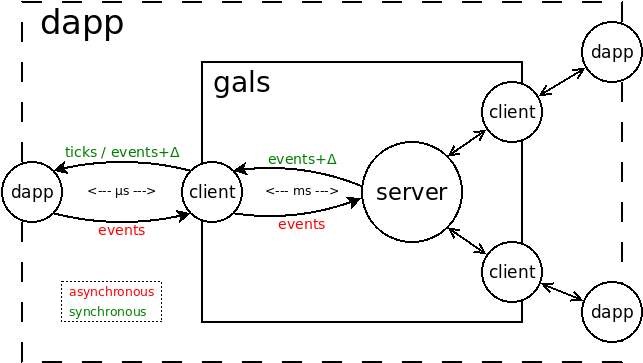
\includegraphics[width=\linewidth]{middleware}
  \caption{
    \label{fig.middleware}
    The architecture of the middleware.
    A single server synchronizes multiple clients, each connected to a mirrored
    instance of the distributed application.
  }
  %\Description{A woman and a girl in white dresses sit in an open car.}
\end{figure}

Events represent user interactions, such as key presses, which are
unpredictable and need to be communicated to the other instances.
Since instances must be indistinguishable from each other by design, event
sources are irrelevant and are ignored.
For instance, if a user presses a key in one instance, the \dapp behaves as if
all users pressed the same key in all instances simultaneously.
%
Clock ticks represent the rate at which applications advance, and are
equivalent to frame rates in video playback and games.
%We assume periods in the order of tens of milliseconds (e.g., 25 milliseconds
%or 40 frames per second).
An important insight is that clock ticks are predictable inputs and need not go
through the server.
This results in no delay between the client and the \dapp since local
interprocess communication takes negligible time.
% (i.e., in the order of a few microseconds).
Otherwise, unlike delays in sporadic mechanical user inputs, users would notice
and condemn delays in clock ticks.
%
Clock ticks and delayed events create a unique synchronous timeline shared by
all instances of the \dapp, making them manifest identical behavior.
Figure~\ref{fig.timeline} is an example of a timeline with asynchronous events
that are synchronized with a delay.
Except for id \emph{0}, which represents clock ticks, applications determine
their event ids, which the middleware just forwards with no further
interpretation.
As detailed in Section~\ref{sec.gals}, the middleware ensures that all
instances receive the same timeline.

\begin{figure}[t]
{\scriptsize
\begin{verbatim}
Tick    Event    Async
----    -----    -----
0000      0
0025      0      --> user presses key (1) and mouse (2)
0050      0
0075      0      --> user presses key (1)
0100      0
0125      1  <-- key is synchronized after delay
0150      0
0175      2  <-- mouse is synchronized after delay
0200      1  <-- key is synchronized after delay
0225      0
0250      0
....     ...
\end{verbatim}
}
  \caption{
    \label{fig.timeline}
    Example of a synchronized timeline of inputs shared by all instances of the
    \dapp.
    Ticks are \emph{25ms} apart (\emph{40 FPS}).
    Asynchronous events are synchronized with a delay.
    Note that delay is unpredictable but event order within each source
    instance is preserved.
  }
\end{figure}

Note that the delay between asynchronous event emission and corresponding
synchronization is inherently nondeterministic due to the network.
An hypothetical re-execution of an application with asynchronous emissions at
the very same ticks would not guarantee that corresponding synchronizations
would have the same delays.
%
However, although a deterministic distributed timeline is impossible to
achieve, our goal is to guarantee a consistent timeline to all instances.
%
More specifically, we propose to extend Lamport's sequential consistency
model~\cite{lamport} with a third property for timing accuracy as follows:
%
\begin{enumerate}
    \item There is a total order of events on which all instances agree.
    \item All events sent from a given instance are received in the same order by others.
    \item All instances receive a given event at the same time.
\end{enumerate}
%
We name this model \emph{timely-sequential consistency} due to the third
property.

%As detailed in Section~\ref{sec.gals}, the delta delay for user input is the
The delta delay for user input is proportional to the maximum RTT considering
all clients.
We deliberately assume unbounded network delay to augment the possible
application scenarios.
Another concern is the rate of input generation in the instances.
As an example, tracking the mouse position will inevitably flood the network
with packets and make applications unresponsive.
For these reasons, the feasibility of applications depends on
    (i) the acceptable delay in the user input,
    (ii) the nature and rate of inputs, and
    (iii) the maximum network latency.

The code for an actual \dapp is the same for all instances and uses a standard
event-driven API with only four commands:
%
\begin{itemize}
\item \texttt{mid\_connect(port,fps)}:   \\Connects with the local client in the given port and desired FPS.
\item \texttt{mid\_disconnect()}:        \\Disconnects with the local client.
\item \texttt{(now,evt) = mid\_wait()}:  \\Waits for the next input carrying a timestamp and event id.
\item \texttt{mid\_emit(evt)}:           \\Emits an event corresponding to an asynchronous input.
\end{itemize}
%
Figure~\ref{fig.skel} shows the skeleton of a distributed application.
The commands \texttt{connect} and \texttt{disconnect} are only required once to
enclose the application logic \lin{2,10}.

\begin{figure}[t]
{\scriptsize
\begin{verbatim}
01  fun dapp (port: Int) {
02     mid_connect(port,40)           // connects to client at 40 FPS
03     while (true) {                 // main event loop
04        val (now,evt) = mid_wait()  // awaits input (every 25ms)
05        switch (evt) {              // reacts to input
06           ...break loop...         //   possibly terminates
07        }
08        ...mid_emit(nxt)...         // possibly generates inputs
09     }
10     mid_disconnect()               // disconnects with the client
11  }
\end{verbatim}
}
  \caption{
    \label{fig.skel}
    The skeleton of a \dapp is a main loop that waits synchronous and emits
    asynchronous events.
  }
\end{figure}

Figure~\ref{fig.timeline}~and~\ref{fig.skel} (the timeline and the program)
relate as follows:
The application initially blocks waiting for an input \lin{4}.
According to the timeline, the first input happens at \emph{tick 0} with
\emph{event 0} (no event).
In the second iteration (\emph{tick 25}), the application emits events \emph{1}
and \emph{2} asynchronously \lin{8}.
Only after a few ticks, these events are synchronized (\emph{ticks 125 and 175})
in the main loop \lin{4}.
As intended, note how the main event loop is coded like a standard local
event-driven application.
We extend this discussion in the next section.

Even though this paper discusses only perfectly symmetric instances, it is
reasonable to support some level of asymmetry in the user interfaces.
For instance, the middleware could provide a \texttt{mid\_self} API to
distinguish between instances, as well as permit that instances react to local
events directly.
However, a proper discussion about the implications is out of the scope of this
paper.

\section{Local Synchronous Programming}
\label{sec.sync}

In the synchronous programming model~\cite{sync}, a program executes in
locksteps (or logical ticks) as successive reactions to inputs provided by an
external environment.
In our context, the environment represents user interactions, and inputs can be
occasional events, such as a key press, or simply the passage of time.
Since execution is guided from outside, the main advantage of the synchronous
model is that it is possible to record a sequence of inputs and reproduce the
behavior of a program multiple times for reasoning and testing purposes.
A fundamental requirement of synchronous programming, known as the
\emph{synchronous hypothesis}~\cite{hypo}, is to isolate logical ticks from
each other to preserve locksteps and prevent concurrent reactions to multiple
inputs, which would break determinism.
This hypothesis can be satisfied if computing reactions is faster than the rate
of external inputs.

An important concern is how to guarantee that isolated reactions are themselves
deterministic and sufficiently fast.
Synchronous languages~\cite{langs} typically restrict the programming
primitives and/or perform static analysis to ensure these properties.
However, since we propose a standard event-driven API targeting generic
programming languages, we assume informally that the programmers themselves
ensure these properties.
This may involve coding best practices, such as avoiding preemptive
multithreading, stateful system calls, and time-consuming loops in programs.

\begin{figure}[t]
  \centering
  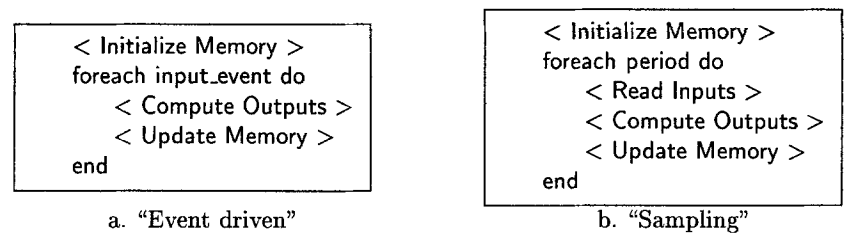
\includegraphics[width=\linewidth]{schemes}
  \caption{
    \label{fig.schemes}
    Equivalent execution schemes for synchronous systems~\cite{schemes}:
    In the first scheme, an event occurrence triggers a loop iteration.
    In the second scheme, a predefined time interval triggers a loop iteration,
    which polls the environment for events.
  }
\end{figure}

Figure~\ref{fig.schemes} shows two common implementation schemes for
synchronous programs~\cite{schemes}.
In both schemes, a loop iteration updates the state of the memory completely
before handling the next input.
Hence, assuming that memory updates are deterministic, the only source of
non-determinism resides in the order of inputs from the environment.
Outputs are asynchronous events in the opposite direction of inputs and
signal the environment about changes.
They typically represent external actuators as opposed to input sensors.

The ``Sampling'' scheme of Figure~\ref{fig.schemes} is very similar to the
\dapp skeleton of Figure~\ref{fig.skel}:
    \texttt{mid\_connect} specifies the sampling period \lin{2},
    \texttt{mid\_wait} reads inputs \lin{4},
    \texttt{mid\_emit} signals the environment back \lin{8}, and
    the \texttt{switch} statement processes the inputs to update memory \lin{5--7}.
As required by the synchronous hypothesis, the sampling period, and
consequently the rate of inputs, must be compatible with the processing speed
of the loop body.
A particularity of our design is that \texttt{mid\_emit} is an output that
corresponds to an asynchronous input that is later synchronized with a delay,
as illustrated in Figure~\ref{fig.middleware}.
%
The sampling scheme of Figure~\ref{fig.schemes} is also adopted by popular
event-driven libraries, such as \emph{SDL} for computer graphics, and
\emph{Arduino} for embedded systems.%
\footnote{SDL: \url{www.libsdl.org}. Arduino: \url{www.arduino.cc}.}
This allows for an easier integration of our middleware with practical systems,
and also reinforces how, in our proposal, programming distributed versions
becomes similar to their local counterparts.

Figure~\ref{fig.sdl} is the code for a \dapp written in SDL to control an
animated rectangle on the screen with the keyboard.%
\footnote {
    Video with two distributed instances: \url{https://youtu.be/HSIwmrUenqg}
}
The code structure follows the synchronous scheme with well delimited regions
to initialize memory \lin{4--8}, read inputs in a loop \lin{11--13}, update
memory \lin{15--28}, and compute outputs \lin{30--31}.
As highlighted in the previous paragraph, outputs correspond to asynchronous
inputs that are later retrofitted into the \dapp.
The output region is expanded in Figure~\ref{fig.input} and is discussed next.
The application first initializes the SDL library to create a window and
renderer handle.
The rectangle starts at position \texttt{(10,10)} with no movement in the axes:
\texttt{vx=vy=0} \lin{7--8}.
The main loop \lin{10--32} first waits for the next input to control the
rectangle \lin{11--13}.
On each iteration, the screen is cleared and the rectangle is drawn on the
current position \lin{15--19}.
The \texttt{switch} statement \lin{20--27} processes the current input:
    a clock tick \lin{21} just moves the rectangle in the current direction;
    a space \lin{22} pauses the rectangle by resetting the axes speeds;
    the arrow keys \lin{23--26} set the axis speeds towards the appropriate direction.
Before the next iteration, the screen is updated \lin{28}.
The code is enclosed by middleware calls to connect and disconnect \lin{2,34}.
Inside the main loop, all state modifications are sequential and depend only on
the received event, which ensures that the application is responsive and
deterministic.

\begin{figure}[t]
{\scriptsize
\begin{verbatim}
01  int main (void) {
02    mid_connect(port, 40); // 25ms ticks
03
04    SDL_Init(SDL_INIT_VIDEO);                 ---\
05    SDL_Window*   win = SDL_CreateWindow();      |
06    SDL_Renderer* ren = SDL_CreateRenderer(win); |> Initialize
07    int x=10, vx=0; // position and              |    Memory
08    int y=10, vy=0; // speed multipler        ---/
09
10    while (1) {
11      uint64_t now;                           ---\
12      uint32_t evt;                              |> Read Inputs
13      mid_read(&now, &evt);                   ---/
14
15      SDL_SetRenderDrawColor(ren, WHITE);     ---\
16      SDL_RenderClear(ren); // clear screen      |
17      SDL_Rect r = { x, y, 10, 10 };             |
18      SDL_SetRenderDrawColor(ren, RED);          |
19      SDL_RenderFillRect(ren, &r); // draw rect  |
20      switch (evt) { // 5px/40fps -> 200 px/s    |
21        case 0:     { x+=5*vx; y+=5*vy; break; } |> Update Memory
22        case SPACE: { vy= 0; vx=0; break; }      |
23        case LEFT:  { vx=-1; vy=0; break; }      |
24        case RIGHT: { vx= 1; vy=0; break; }      |
25        case UP:    { vy=-1; vx=0; break; }      |
26        case DOWN:  { vy= 1; vx=0; break; }      |
27      }                                          |
28      SDL_RenderPresent(ren);                 ---/
29
30      // emit asynchronous inputs             ---\  Compute Outputs
31      ... mid_emit(evt) ...                   ---/
32    }
33
34    mid_disconnect();
35    return 0;
36  }
\end{verbatim}
}
  \caption{
    \label{fig.sdl}
    A \dapp in SDL to control an animated rectangle on the screen with the keyboard.
  }
\end{figure}

Figure~\ref{fig.input} expands the output region with calls to
\texttt{mid\_emit} that generate asynchronous inputs.
In this application, the code simply calls the SDL library to check whether a
key is pressed to forward it to the middleware. % (\emph{ln. 11--13} in Figure~\ref{fig.sdl}).
Note that in a local-only application this region of code would replace the
region to read inputs from the middleware.
Note also that it is not necessary to customize this code for every single
\dapp.
Instead, the middleware may provide a custom input generation stub for each
event-driven library it supports, which \dapps can reuse.
This is the reason why we split this code in a separate figure.

\begin{figure}[t]
{\scriptsize
\begin{verbatim}
// emit asynchronous inputs
SDL_Event inp;
if (SDL_PollEvent(&inp)) {
   if (inp.type == SDL_KEYDOWN) {
      switch (inp.key.keysym.sym) {
         case SDLK_LEFT:  { mid_emit(LEFT);  break; }
         case SDLK_RIGHT: { mid_emit(RIGHT); break; }
         case SDLK_UP:    { mid_emit(UP);    break; }
         case SDLK_DOWN:  { mid_emit(DOWN);  break; }
         case SDLK_SPACE: { mid_emit(SPACE); break; }
      }
   }
}
\end{verbatim}
}
  \caption{
    \label{fig.input}
    Asynchronous input generation with \texttt{mid\_emit}.
    The library polls for key presses and forwards them to the middleware.
  }
\end{figure}

To conclude this section, the ``Update Memory'' region of Figure~\ref{fig.sdl}
\lin{15--28}, which contains the core logic of the application, does not make
calls to the
middleware, being indistinguishable from a local version.
In addition, since this region complies with the synchronous model premises,
the application remains responsive and deterministic.
For instance, the computations to update the positions are clearly faster than
\emph{25ms} (a tick period), satisfying the synchronous hypothesis.
Also, if a timeline such as that of Figure~\ref{fig.timeline} is applied to
multiple re-executions of the application, then the sequence of memory updates
to \texttt{x}, \texttt{y}, \texttt{vx}, and \texttt{vy} \lin{20--27} will be
identical in every single execution.
In the next section, we discuss how to extend these guarantees to a distributed
setting.

\section{The Synchronization Protocol}
\label{sec.gals}

The synchronous programming model assumes a single clock that controls the main
loop to update the application state in locksteps.
However, when we distribute the \dapp in multiple instances, we can no longer
assume a single clock source, which compromises the synchronous hypothesis.
% we introduce a delay due to communication, and
%
Nevertheless, in order to guarantee identical behavior to symmetric distributed
applications, we need to read perfectly synchronized inputs in real time in all
instances.
For example, in the rectangle application of Figure~\ref{fig.sdl}, the
challenge is to broadcast and then resynchronize all asynchronous calls to
\texttt{mid\_emit} \lin{31}, so that calls to \texttt{mid\_read} \lin{13} awake
at the same time in all instances.

In the ``Globally-Asynchronous Locally-Synchronous Architecture'' (GALS),
independent synchronous processes communicate asynchronously through the
network~\cite{gals.taxonomy}.
Since processes are locally synchronous, asynchronous communication is the only
source of nondeterminism.
%
Inspired by the simplicity of GALS, we want not only to keep the local
guarantees of synchrony, but also to extend them globally, by transferring the
responsibility of dealing with asynchrony to the middleware.
%
As illustrated in Figure~\ref{fig.middleware}, \dapp local instances depend on
synchronous inputs only (green arrows), and are allowed to output asynchronous
events (red arrows).
%
However, unlike traditional GALS, the middleware automatically resynchronizes
inputs in a single global timeline so that all instances observe them
identically.
Hence, the middleware must satisfy the timely-sequential consistency model for
distributed timelines described in Section~\ref{sec.arch}.

Resynchronization adds a delta delay to the original event that is proportional
to the maximum RTT considering all clients.
The reason for this is that the synchronization protocol needs to consider two
main issues:
%
\begin{itemize}
\item \textbf{Clock differences:}
    Each instance has an independent clock that differs from others in
    \emph{offset} and \emph{rate}.
    The offset corresponds to the absolute point in time since the \dapp started.
    As an example, suppose one instance started \emph{5000ms} ago while another
    started \emph{5051ms} ago.
    The \emph{rate} corresponds to how fast the clock progresses, which may
    slightly differ between machines.
    As an example, suppose one instance misses \emph{25ms} every hour in
    comparison to others.
    This difference, aka clock drift, may affect the \emph{offset} considerably
    over time.
\item \textbf{Network delay:}
    Instances are subject to communication delays with the server, which vary
    between clients and also over time.
    As an example, suppose a client next to the server has a stable RTT of
    \emph{10ms}, while for a distant one, RTT may vary between \emph{50--100ms}
    over time.
\end{itemize}
%
In our synchronization protocol, we do not assume any strict bounds in clock
differences and network delays, which may of course affect the feasibility of
some applications.
%
The protocol has the following goals:
%
\begin{enumerate}
\item Ensuring that instances read inputs with perfect time accuracy.
\item Generating synchronous inputs back to instances with minimum delays.
\item Keeping clock offsets at instances close to each other.
\end{enumerate}
%
Regarding \emph{goal~3}, offset differences are inevitable but should be under
a few milliseconds to be unnoticed by users.
Regarding \emph{goal~2}, the smaller the input delay, the better is the user
experience regarding interactivity.
However, if too small, a distant instance may receive the delayed input after
its local time, which is unacceptable considering \emph{goal~1}.
In this case, the client freezes its associated instance pausing the local time
to ensure time accuracy, which is our ultimate goal.

It is important to recognize that an instance cannot by itself determine a
reasonable timestamp for an event and broadcast it directly to others:
%
First, the client has no idea about the network RTT to guarantee that all other
clients would receive the event in time to fulfill \emph{goal~1}.
%
Second, even if known, there is no guarantee that the RTT will not slightly
increase momentarily, causing an instance to miss the event deadline.
%
Third, even if the RTT was known and bounded, local instances might still
diverge on local time offsets (since they advance independently), again causing
an instance ahead in time to miss the deadline.
%
Hence, our protocol relies on a central server to determine a reasonable
timestamp for all clients, and to ensure that instances do not miss deadlines
even if everything goes wrong.

Figure~\ref{fig.protocol} describes the synchronization protocol performed by
the middleware.%
\footnote {
    Video with two distributed instances, now with deliberate RTTs in the order
    of \emph{100ms}: \url{https://youtu.be/bf9C2mwkTzA}
}
The next paragraphs explains the protocol in detail.

\begin{figure}[t]
  \centering
  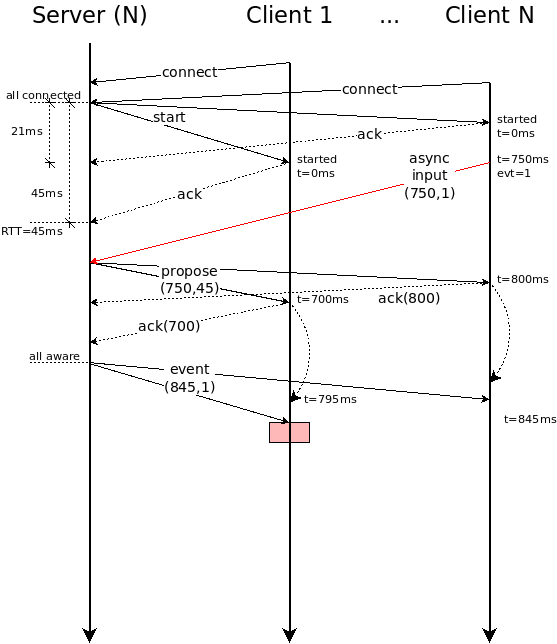
\includegraphics[width=\linewidth]{protocol}
  \caption{
    \label{fig.protocol}
    The synchronization protocol
        (i) keeps clock offsets together,
        (ii) generates synchronous inputs with minimum delays, and
        (iii) ensures that instances read inputs with accuracy.
  }
  %\Description{A woman and a girl in white dresses sit in an open car.}
\end{figure}

The server starts first and needs to know in advance how many instances will
participate in the \dapp (\emph{Server (N)}).
Each instance connects through its client (\emph{Client~1 ... Client~N}) to the
server, which in turn waits for all connections to succeed
(\emph{all connected}).
Then, the server broadcasts a \emph{start} message to all clients, which on
receipt, start sending clock ticks to their instances (\emph{started}).
Note that clients will inevitably start at different absolute times due to
network latency.
The clients also send back an \emph{ack} so that the server can calculate the
maximum network RTT (\emph{RTT1=45ms}), which is used next.
%
After the startup process, each \dapp instance executes at the same pace
(except for drifts) with similar offset differences (at most \emph{RTT1}).
At this point, we consider instances to be indistinguishable from each other.

Now, let's consider an asynchronous event (in red).
%
Since clients cannot determine a reasonable timestamp, \emph{Client~N} emits
\emph{evt=1} towards the server at local time \emph{750ms} (\emph{async(750,1)}).
%
The server enqueues all requests and handles each event atomically, in
sequence, as follows:
%
First, it broadcasts the intention to emit an event (\emph{propose(750,45)}),
passing the source instance offset time (\emph{750ms}) and current overall RTT
(\emph{RTT1=45ms}).
Before it broadcasts the synchronous event with the final deadline
(\emph{sync(895,1)}), each client calculates its own deadline as follows:
    (i)   takes the maximum time between the source and local offset,
    (ii)  adds twice the received RTT,
    (iii) adds a small constant time (\emph{5ms}),
    (iv)  sets this sum as the local event deadline.
As examples, the sum for
    \emph{Client~1} is $max(750,700)+2x45+5=845$, and for
    \emph{Client~N} is $max(750,800)+2x45+5=895$.
%
This sum is reasonable because it takes into account
    the instance most ahead in time, and also
    the worst RTT with an extra margin.
For instance, \emph{Client~N} with the worst RTT (\emph{45ms}) is also ahead of
time (\emph{800ms}) and the final event will arrive after another round trip to
the server, thus making \emph{895ms} a reasonable deadline.
%
The small constant depends on the number of instances in the application and is
currently set to 200us per instance (e.g., \emph{5ms} for \emph{25} instances).
%
During this process, the server also recalculates the RTT to use in the next
event emission (\emph{RTT2=50ms}).

Each client also starts a timer to freeze the instance if the (now expected)
synchronous event is not received until its local deadline.
In this case, the client pauses the instance by repeating the same clock tick
over and over, until it receives the event.
Although unfortunate, this at least ensures identical timelines in all
instances to comply with \emph{goal~1}.
%
The server then waits for all client \emph{acks} carrying their local offsets
(\emph{ack(700)} and \emph{ack(800)}), recalculates each deadline (in the same
way each client did), and takes the largest as the final event timestamp to
broadcast to all clients (\emph{sync(895,1)}).
We emphasize here that the server needs to wait for \emph{all clients} and take
into account their local times to ensure that the final timestamp is suitable
to all clients.
This is a severe limitation, which we discuss further, because the protocol
halts with a single client failure.
%
The server also sends drift compensations (\emph{dt(100)} and \emph{dt(0)})
based on offset differences between clients (we will discuss this later).
At this point, all clients are expecting a timestamp that is greater than or
equal to their own timer deadlines.
Therefore, even if the network deteriorates, no instances will miss the
synchronized event because they will be frozen before their deadlines.

Finally, the expected synchronous event is received by the clients
(\emph{sync(895,1)}).
\emph{Client~N} receives it before the deadline, at local time \emph{870ms},
requiring it to postpone local emission for another \emph{25ms} to match the
event timestamp with perfect accuracy (\emph{895ms}).
However, the timer at \emph{Client~1} expires before receipt, requiring it to
freeze the \dapp for a while (red area).
Then, the synchronous event is received at local time \emph{860ms}, but still
requires another \emph{35ms} to match its timestamp.
In the end, both clients emit the event exactly at local time \emph{895ms} as
expected (white circles).

Note that \emph{Client~1} was harmed in the process mainly because its maximum
time of \emph{750ms} was much smaller than the \emph{800ms} for \emph{Client~N}.
This is because the local clocks were too distant from each other, breaking our
\emph{goal~3}.
Note also that pausing \emph{Client~1} increased the offset difference even
further (\emph{offset diff}).
%
The middleware also implements an algorithm to compensate clock drifts as
follows:%
\footnote {
    Video with two distributed instances, now with exaggerated clock drifts:
    \url{https://youtu.be/wwlAURjN5YY}
}
Once the server receives all acknowledgments carrying local offsets
(\emph{ack(700)} and \emph{ack(800)}), the server sends back how much each
client is behind in comparison to the maximum value (i.e., \emph{800-700=100}
and \emph{800-800=0}).
If this number is greater than zero, the client speeds up each local tick in
\emph{20\%} until the time drift is compensated.
For instance, if the client behind generates new ticks every \emph{25ms}, it
will instead generate \emph{25ms} ticks every \emph{20ms} for a while.

In order to maintain the overall network RTT updated and the clock offsets
close to each other, the first client to connect with the server sends a
heartbeat null event (\emph{id=0}) every \emph{5 seconds} to kick off the
synchronization protocol automatically%
\footnote {
    Video with two distributed instances, now with random RTTs, clock drifts,
    and periodic synchronization:
    \url{https://youtu.be/BYNHGsHnMx8}
}.

As mentioned above, each asynchronous request is enqueued according to server
receipt order and is handled atomically, which includes associated roundtrips
to clients.
Hence, original local offsets in requests from different clients may be
handled out of order.
This is not a problem because final timestamps are guaranteed to remain in
order since they depend on the maximum local times collected after each
atomic request.

As the main limitations,
    (1) our protocol does not accept new clients, and
    (2) clients must be responsive during the entire \dapp execution.
%
To address the first limitation, the server could keep the global timeline of
synchronized events in memory and redirect it to new clients as they join,
which then need to apply the events locally to reach the same state of other
clients.
%
To address the second limitation, the server could set an arbitrary waiting
limit (e.g., 2 seconds) to kick out a client from the session and restore
progress in the protocol.
The kicked client would need to restart itself, rejoin the session and,
re-execute the whole timeline.
%
%It should also be possible to take snapshots of the application state to
%optimize session joins, which impose limitations in the programming data structures.
%
Nevertheless, the core of the synchronization algorithm described in
Figure~\ref{fig.protocol} still makes these assumptions and would not be
affected by the changes.

In the next section, we evaluate the performance of the protocol%
\footnote {
    Video with 100 distributed instances running in the Localhost:
    \url{https://youtu.be/in5sdEEyGik}
}.

\section{Evaluation}
\label{sec.eval}

We present the protocol evaluation taking into consideration its main goals:
%
\begin{enumerate}
\item Ensuring that instances read inputs with perfect time accuracy.
\item Generating synchronous inputs back to instances with minimum delays.
\item Keeping instances clock offsets close to each other.
\end{enumerate}
%
In order to verify if these goals are met, we created a series of experiments
to measure the properties as follows:
%
\begin{itemize}
\item \textbf{Clock drift}:
    the percentage of drift compensation relative to the total simulation time
    (i.e., $1\%$, if drifts accumulate $1s$ in $100s$).
\item \textbf{Event latency}:
    the average number of frames elapsed from asynchronous emits to their
    corresponding synchronous receipts (e.g., $3$, if an emit occurs at frame
    $58$ and receipt at $61$).
\item \textbf{Frame freeze}:
    the percentage of repeated frames relative to the total simulation frames
    (i.e., $1\%$, if $1$ frame freezes every $100$ frames).
\begin{comment}
\item \textbf{Frame late}:
    the percentage of frame delays due to CPU load relative to the total
    simulation time (i.e., $1\%$, if delays accumulate $1s$ in $100s$).
\end{comment}
\end{itemize}
%
%The evaluation is detailed in Figure~\ref{fig.table}.
%
Drift compensation ensures that clock offsets are kept closer (\emph{goal~3}),
but a high percentage of clock drift may indicate that the protocol is actually
causing it.
Ideally, clock drift rate should be $0\%$.
%
A high event latency may compromise \emph{goal~2}, but a low latency may
increase the amount of frame freezes, which is even less desirable.
Ideally, event latency should be $1$ frame, and freeze rate, $0\%$.
%
\begin{comment}
As an implicit goal, the applications preserve their original frame rates when
going distributed.
The protocol should not affect this property (and vice versa).
Ideally, frame late rate should be $0\%$.
However, in our experiments, we simulate a CPU load between \emph{50--110\%} to
stress the protocol.
%Hence, ideally, late rate should be around $TODO\%$.
\end{comment}
%
Note that \emph{goal~1} is a strict requirement, which the protocol ensures
with 100\% accuracy by design.
In this sense, our experiments log the timelines of all instances and just
asserts that they are identical in all simulations, since this is the only
possible result.

We simulated a variety of scenarios with the following factors:
%
\begin{itemize}
\item \emph{NET} (network connection type):
    affects network RTT.
\item \emph{FPS} (application frame rate):
    affects client CPU load.
\item \emph{N} (number of instances in the network):
    affects network traffic and server CPU load.
\item \emph{Rate} (rate of inputs):
    affects network traffic and client/server CPU load.
\end{itemize}
%
\begin{comment}
For instance, for a video game with a few friends over the LAN, the parameters
could be
    \emph{3--5} instances,
    an RTT of \emph{5--10ms},
    FPS around \emph{50},
    and a new interaction around every \emph{500ms}.
\end{comment}
As an example of a concrete scenario, an interactive class over the Internet
could have
    an RTT of \emph{50--200ms} (\emph{NET}),
    execute at \emph{25} frames per second (\emph{FPS}),
    with \emph{50} instances (\emph{N}),
    interacting every \emph{5s} (\emph{Rate}).
%e.g., a slide advance).

For each of these four factors, we tested the following values:
%
\begin{itemize}
\item \emph{NET}: \emph{Loopback}, \emph{LAN}, and \emph{WAN} (\emph{0--50ms} RTT).
                                                                 % 3
\item \emph{FPS}: $10$, $25$, $50$, $100$ frames per second.     % 4
\item \emph{N}: $2$, $5$, $10$, $25$, $50$, and $100$ instances. % 6
\item \emph{Rate}: $5s$, $1s$, $500ms$, and $250ms$ period between events.
\end{itemize}                                                    % 4
%
These values result in $288$ combinations.
We executed each combination $3$ times for $5$ minutes each.
The experiments take $72$ hours to complete.

\begin{figure*}[t]
  \centering
  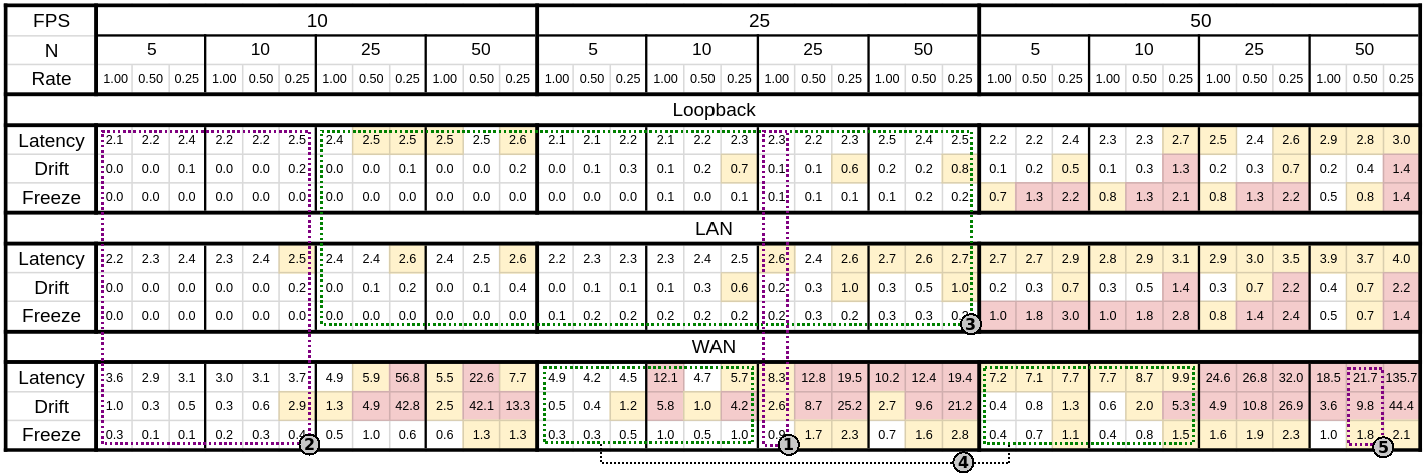
\includegraphics[width=\linewidth]{table2}
  \caption{
    \label{fig.table}
The \emph{Loopback}, \emph{LAN}, and \emph{WAN} regions each contains $36$
measures for multiple configurations of $FPS$, $N$, and $Rate$.
The rate of inputs appears in \emph{seconds per events}, e.g., $0.50$ means two
events per second.
%
The color thresholds (\emph{yellow},\emph{red}) vary between WAN and local
networks (LAN/Loopback) and are as follows:
    \emph{Latency} (Local: 2.5,5 ; WAN: 5,10);
    \emph{Drift}   (Local: 0.5,1 ; WAN: 1,3);
    \emph{Freeze}  (Local: 0.5,1 ; WAN: 1,3).
The threshold values are arbitrary but help to distinguish between regions of
interest.
%
The \emph{Loopback} experiments used a single machine with $1$ process for the
server, $N$ processes for the clients, and $N$ processes for the \dapp
instances.
The \emph{LAN} and \emph{WAN} experiments used a machine dedicated for the
server, and $3$ other machines each with $N/3$ processes for the clients and
instances.
%
The experiments use heterogeneous \emph{Linux} distributions with the machine
configurations as follows:
    \emph{Loopback} (\emph{i7/8GB});
    \emph{LAN} (server \emph{i7/8GB}; clients \emph{i7/16GB}, \emph{i7/8GB}, \emph{i5/4GB});
    \emph{WAN} (server \emph{Xeon-VM/1GB}; clients \emph{2x i7/8GB}, \emph{i5/4GB}).
  }
  %\Description{A woman and a girl in white dresses sit in an open car.}
\end{figure*}

Figure~\ref{fig.table} shows a summary with $108$ out of all $288$ measures.
We omit \emph{N=2}, \emph{N=100}, \emph{FPS=100}, and \emph{Rate=5s} to save
space in the figure and because they do not affect the discussion that follows.
The color of the squares indicates their performances
    (white=good, yellow=moderate, and red=poor).

The thin vertical rectangle labelled \textbf{1} in the figure highlights an
experiment running at $25$ FPS, with $25$ simultaneous instances, generating an
event every second.
%
The results show that this scenario is viable in all network configurations,
including WAN:
%
The latency around $8$ frames means that an instance broadcasts an asynchronous
event and applies it synchronized $330ms$ later, in the average.
The drift of $2.6\%$ means that for every minute of execution in each instance,
the middleware needs to compensate $1500ms$.
The two frozen frames of $0.9\%$ means that for every $2400$ frames
($1$ minute), $20$ frames are repeated.
%Late frames correspond to $0.67\%$, i.e., $16$ frames in $1$ minute.
%
Unsurprisingly, the results for local networks with the same factor levels are
better, specially latency and drift.

Rectangle \textbf{2} indicates a safe region for all network types: up to $10$
FPS, $10$ instances, and $4$ events per second.
%
Rectangle \textbf{3} indicates a safe region for LANs: up to $25$ FPS, $50$
instances, and $4$ events per second.
%
The worst measured averages in these two large regions are
    a $2.7$ latency in the LAN ($110ms$),
    a $2.9\%$ drift and
    a $0.4\%$ freeze over the WAN.
%
Therefore, we can conclude that low frame-rate applications ($10$ FPS), with
reasonable network size ($10$ instances) and high activity ($4$ events per
second) can be reliable even over the WAN.
For LANs, the reliability reaches high frame rates ($50$ FPS) and a larger
network size ($25$ instances), which is enough even for video games in a local
network.

Rectangles \textbf{4} indicate a region of interest for WANs: up to $50$ FPS
and $10$ nodes.
The worst measured averages in these rectangles are
    a $12.1$ latency ($500ms$),
    a $5.8\%$ drift, and
    a $1.5\%$ freeze.
This is a high frame rate region that admits a reasonable number of nodes,
possibly with low event latency, which is enough for applications such as
family watch parties over the Internet.

The other squares in the figure should be considered in isolation and depend on
the target application and its requirements.
%
As an example, let's consider rectangle \textbf{5}: $50$ FPS, $50$ instances,
and $2$ events per second for the WAN.
A $21.7$ latency corresponds to almost $1$ second, but this might still be a
reasonable delay for many applications.
A drift of $9.8$ means that the server will be constantly, but smoothly,
compensating the instances clocks.
A freeze below $2\%$ over the Internet is also a reasonable value.

\begin{comment}
- RTT (para ver se bate com estilo da rede)
- Latencia/Delay (entre async/sync)
    - O minimo seria 2RTT+DT/2 por conta do protocolo
    - O minimo teorico seria RTT/2 em media, que é o tempo de bcast de um evento
- Relacao entre RTT e latencia

% - what ifs c/ videos
% - revisitar limitacoes e propor alternativas na secao de avaliacao
% - Need total order in real time. Ok leader, raft, etc, not ok Blockchain
\end{comment}

\begin{comment}
\section{Asymmetric Distributed Applications}

\begin{itemize}
\item precisa de nao determinismo para mudar comportamento
\item nao determinismo se resuma a uma unica nova API: gals-self-nondet()  <-- retorna ID local
\item assimetria se reduz em "if (gals-self-nondet() == xxx) ..."
\item cuidados para os ifs apenas serem para geração de eventos (controle 1, controle 2, etc) e view local (TV, controle, etc)
\end{itemize}

With distribution, communication timing is asynchronous because communication
latency takes a non-negligible time and breaks the synchronous hypothesis.
What about in realtime
- a perfect mirror, cannot distinguish
- high-level vs low-leve events, semantic events
    - more abstract solves both problems (delay and rate)
- clear/sound properties to reason
- Events: single application, multiple views, may restrict events per node
    - gals\_self()

Concurrent programs in non-deterministic languages are notoriously hard to prove correct and have led to well-known disasters.

\section{Applications}
\label{sec.apps}

\subsection{Symmetric Video Playback}

\begin{itemize}
\item mesmo video e interface em todas as instancias
\item clique de "pause" tem efeito no mesmo frame de todas as instancias
\item stub do gstreamer controlado frame a frame
\end{itemize}

\subsection{Asymmetric Graphics Editor}

\begin{itemize}
\item editor retangulos (cria, redimensiona, move)
\item dois cursores "assimétricos"
\item precisa de eventos de alto nivel (provavelmente nao dá pra manter a posicao dos mouses em tempo real)
\end{itemize}
\end{comment}

\section{Related Work}
\label{sec.related}

Synchronous languages~\cite{langs} focus on static guarantees for critical
real-time control systems.
They are based on a well-behaved lockstep execution that simplifies reasoning
and verification of programs.
They also restrict control and data primitives to enforce determinism and
static bounds on memory usage and execution time.
On the one hand, these guarantees enforce identical behavior to local instances
in symmetric distributed application.
On the other hand, the restrictive semantics of synchronous languages hinders
the development of rich collaborative applications.
We chose a pragmatic approach and provide a standard event-driven API with no
restrictions.
Nonetheless, this API can support host environments in synchronous languages.

In GALS architectures~\cite{gals.taxonomy}, computations within local
synchronous nodes are deterministic, with communication latency being the only
global source of nondeterminism.
We propose a middleware to tame nondeterminism and provide global sequential
consistency to all nodes.
%
Some programming languages and systems~\cite{gals.crp,gals.crsm,gals.systemj}
expose the GALS architecture to programmers, but still leave to them the
responsibility to coordinate interprocess communication over the network.
%
Concurrent Reactive Processes (CRP)~\cite{gals.crp} extend the synchronous
language Esterel~\cite{esterel} with asynchronous communication
channels resembling CSP~\cite{csp}.
%
Esterel enforces determinism and bounded reactions to local instances, which
are linked by asynchronous channels.
Instances are asymmetric in the sense that they may execute different
applications.
Also, there is no central coordination towards a consistent global timeline,
and each instance advances its clock independently.
%
CRSM~\cite{gals.crsm} and SystemJ~\cite{gals.systemj} are similar systems, with
CSP-like asynchronous channels and Esterel-like synchronous lockstep execution.
The main difference to CRP is that they use Argos~\cite{argos} (CRSM) and Java
(SystemJ) as their local programming languages.

``Physically Asynchronous Logically Synchronous Systems (PALS)''~\cite{gals.pals}
is a synchronization protocol to support strict real-time distributed
applications.
PALS provides a perfectly synchronized global clock shared by all instances,
which leads to identical state transitions in all instances.
%
On the one hand, PALS provides stronger synchrony in comparison to our
protocol.
In our proposal, local clocks advance independently and events need to be
delayed to fit all instances timelines, possibly resulting in application
freezes.
%
On the other hand, PALS requires stronger assumptions, namely bounded limits
for clock skews, network latency, and local computation time.
We support unbounded limits that only affect the viability of applications in
certain scenarios.
%
Our protocol also keeps the instance clocks close to each other, but not as a
strict real-time constraint.
This is enough to keep the instances indistinguishable to the human eyes, and
not affect the prediction of input delays.
%
Regarding the protocol implementation, PALS also relies on a central server to
serialize the timeline, but delivers a lower event latency.
Since the bounds are fixed and known in advance, and all instances are
at the same logical tick, PALS can skip the ``proposal round'' required by our
protocol.

Croquet~\cite{croquet} is a 3D collaboration architecture and dynamic
programming environment with a synchronization protocol called \emph{TeaTime},
which more recently became a product%
\footnote{Croquet.io: \url{https://croquet.io/}}.
Croquet relies on a similar centralized architecture to our work, but takes
advantage of the cloud to place the server as close to clients as possible for
better performance.
In contrast to our work, Croquet relies on the server to issue tick events to
clients, which gives full control of the timeline.
The server also timestamps events coming from the clients and redirect them to
all participants.
This results in a simpler protocol that supports joins and leaves
transparently, and does not require roundtrips to determine timestamps.
However, since all tick messages need to be transmitted in the network, the FPS
rate of applications is proportional to the network latency.
For instance, a latency of \emph{100ms} supports at most \emph{10 FPS}.
The transmission of ticks at higher FPS rates also incur in higher network
traffic and server load.
Another distinction between the protocols is that Croquet favors instances with
better latency, which have optimal experience.
In contrast, our protocol adjusts event latency dynamically to accommodate the
slower instance.
In addition, instances execute at the same tick rate respecting local times,
regardless of the network latencies.

Alternative approaches for distributed symmetric behavior include consensus
algorithms and conflict-free data structures towards eventual consistency.
Both approaches have the advantage that instances can apply inputs locally
with immediate feedback.
%
However, consensus algorithms may reorder events, which requires that
operations are reversible or that instances keep snapshots of the application
state to rollback and reapply events in new orders.
Photon%
\footnote{Photon engine: \url{https://www.photonengine.com}}
is an industry networking engine and multiplayer platform that supports
snapshots and rollback.
%
Conflict-free replicated data types (CRDTs)~\cite{crdts} take a data-centric
approach.
Instead of hiding the data in the applications and only communicating events to
transform the data, CRDTs expose data transformations in ways that they may
occur concurrently with the guarantee that they are merged automatically and
reach the same state.
One advantage is that applications work offline with the same
guarantees~\cite{local}.
A disadvantage is that typical data structures are not CRDTs, which requires
that applications are designed carefully around specialized data structures.
%
Our work enforces sequential consistency, which ensures that events are never
reordered, making rollbacks and CRDTs unnecessary.
However, instances need to be always connected and they cannot apply events
locally to support immediate feedback.

\section{Conclusion}
\label{sec.conclusion}

In this work, we propose \emph{Symmetric Distributed Applications} as mirrored
application instances that can broadcast inputs to each other and yet conform
to identical behavior.
%
Using a standard event-driven API, programmers write code as if the application
executes in a single machine.
Our middleware intercepts event generation and synchronizes all instances with
a delay in a consistent timeline, so that receipt is identically reproducible.
%
Not only distributed applications benefit from consistency and determinism but
also development and testing can be done in a single instance with the same
guarantees.

The middleware is based on a GALS architecture, in which nodes are locally
deterministic, but subject to a global source of nondeterminism due to network
latency.
However, unlike traditional GALS, our middleware automatically resynchronizes
inputs in a single global timeline so that all instances observe them
identically.
The middleware satisfies the timely-sequential consistency model, which extends
sequential consistency with timing accuracy.
%The middleware needs to handle clock differences between instances as well as
%latency variations in the network.
%The middleware keeps the instance clocks close to each other, generates
The synchronization protocol works in two phases when receiving an asynchronous
input:
First, it asks the clients for a reasonable deadline, which also prepares them
for the exact incoming timestamp.
Next, the middleware collects all client responses and sends the synchronized
event back to clients.

We evaluated the performance of the protocol with a series of experiments
varying the network latency and size, and the application frame and event rate.
%
We highlighted a reliable and high-performant region of parameters of up to
$10$ FPS and $10$ instances for WANs, and of up to $25$ FPS and $50$ instances
for LANs.
We also identified a region of interest for WANs of up to $50$ FPS and $10$
nodes, but with an event latency in the order of $500ms$.
%
The protocol evaluation helps identifying the distributed application scenarios
that the middleware can handle.

\bibliographystyle{ACM-Reference-Format}
\bibliography{rebls-21}

\end{document}
\endinput
